% !TeX spellcheck = ru_RU
% !TEX root = vkr.tex

\section{Исследование производительности tokio}

Целями данной главы является изучение изменения производительности при разделении константного количества исполнителей между различным количеством инстансов асинхронных рантаймов: если синхронизации исполнителей накладывают ограничение на производительность системы, использующей один асинхронный рантайм, использование нескольких асинхронных рантаймов с меньшим количество исполнителей и должно продемонстрировать большую пропускную способность.

\subsection{Условия экспериментов}\label{experiment_environment}

Для измерения производительности была использована библиотека \verb|criterion|\footnote{\href{https://github.com/bheisler/criterion.rs}{Репозиторий} проекта criterion (Дата обращения: 4.1.2025)}. Так как она популярна, имеет обширную документацию и используется в \verb|tokio|.

Здесь и далее эксперименты производились при следующих условиях:

\begin{itemize}
    \item Исследования проводились на системе YADRO VEGMAN Rx20 G2\footnote{\href{https://yadro.com/ru/vegman/rx20g2/specs}{Описание} системы YADRO VEGMAN Rx20 G2}.
    \item Бенчмарк был запущен со значением \verb|nice| равным минус двадцати.
    \item Исполнение было рекомендовано на одной NUMA единице с помощью \verb|taskset|.
\end{itemize}

Машина для измерения производительности была предоставлена командой \verb|TATLIN.BACKUP| и использовалась удаленно, в связи с чем на ней было невозможно отключение сети.

Библиотека \verb|criterion| имела следующую конфигурацию:

\begin{itemize}
    \item Пять секунд прогрева.
    \item Сорок семплов для каждого измерения.
    \item Линеаризация в качестве способа семплирования.
\end{itemize}

\subsection{Ход исследования}

Для проверки гипотезы об ограничении производительности ресурсами одного рантайма, были произведены измерения пропускной способности системы, состоящей из нескольких рантаймов, приведенные на графике \ref{fig:tatlin:multi_rt:eval}. Каждое измерение использовало одинаковое количество потоков исполнителей и задач производителей, равномерно разделенных между рантаймами.

\begin{figure}[H]
    \begin{center}
        \makebox[\textwidth]{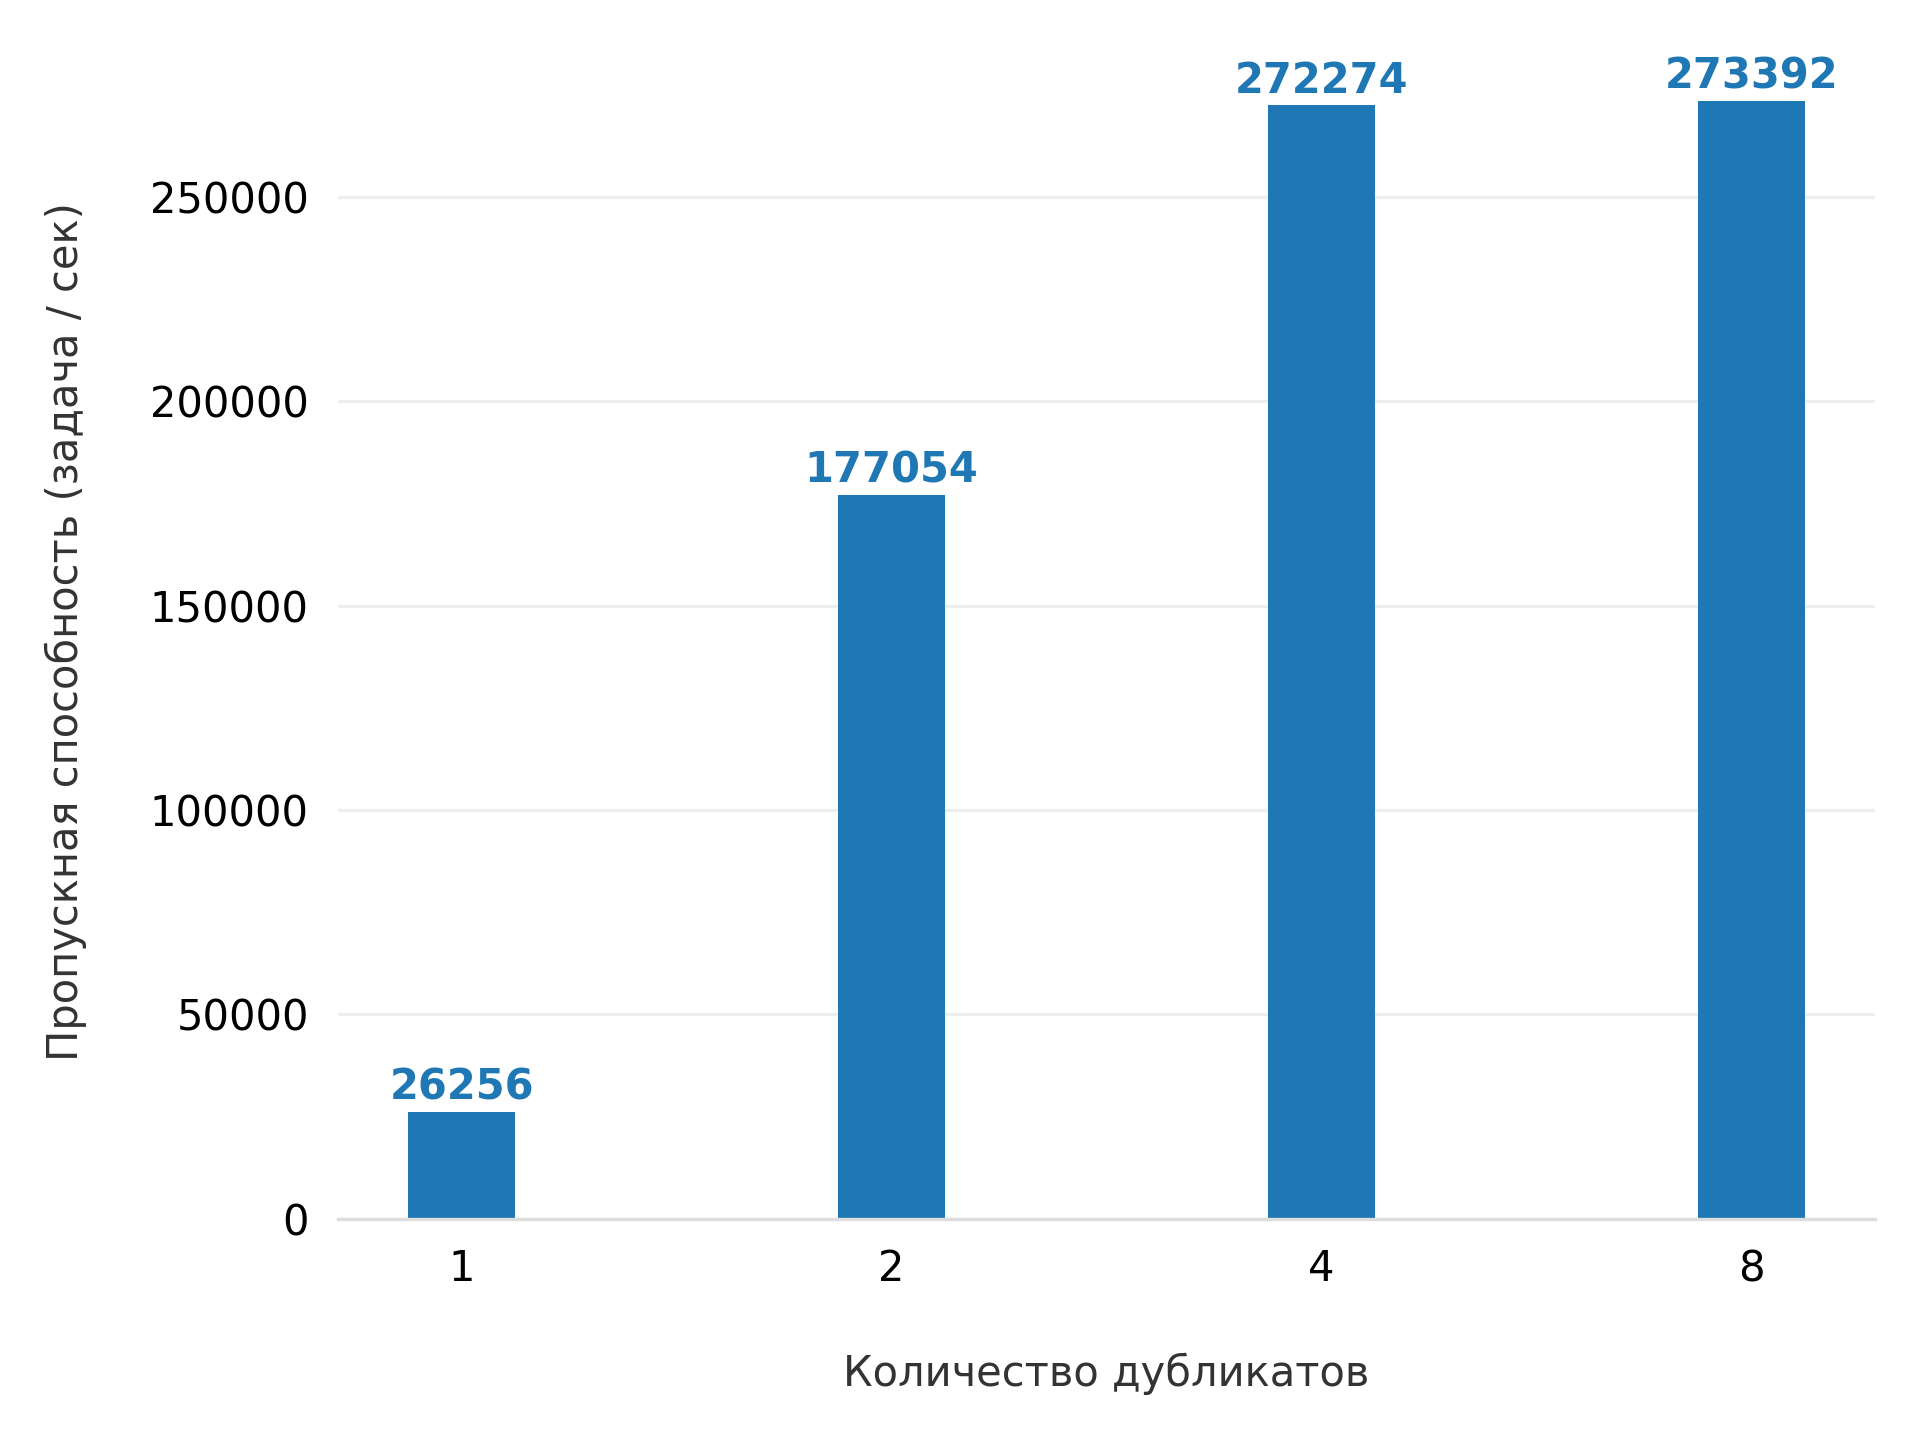
\includegraphics[scale=0.90]{pictures/rt_nsapwner128_nspawn1000.png}}
    \end{center}

    \caption{Производительность системы при использовании нескольких рантаймов.}
    \label{fig:tatlin:multi_rt:eval}
\end{figure}

Из изображения заметным становится увеличение производительности при увеличении количества рантаймов, то есть разделение задач между меньшими изолированными группами исполнителей позволяет увеличить пропускную способность.

\subsection{Вывод}

При изоляции меньших групп исполнителей с отдельными глобальными очередями в рамках отдельных инстансов рантаймов наблюдается увеличение пропускной способности. Это может происходить из-за уменьшения количества синхронизаций между исполнителями:

\begin{itemize}
    \item Меньшая борьба за глобальную очередь, за счет деления исполнителей между несколькими очередями.
    \item Меньшее количество исполнителей пытаются украсть задачи у соседей из-за изоляции исполнителей в различных инстансах рантайма.
\end{itemize}

Таким образом, шардирование рантайма позволяет увеличить пропускную способность системы.
